\documentclass{article}
  %----------------------------------------------------------------------------------------
%	Author:	WangYifu
%	Create Date:	2017-02-14
%	Last Modify:	2018-09-01
%----------------------------------------------------------------------------------------
\usepackage[T1]{fontenc}
\usepackage{fourier}
\usepackage[english]{babel}
\usepackage{amsmath,amsfonts,amsthm}
\usepackage{geometry}
\usepackage{fancyhdr}
\usepackage{listings}
\usepackage{color}
\usepackage[yyyymmdd]{datetime}
\usepackage{graphicx}
\usepackage{float}
\usepackage{titling}
\usepackage{titlesec}
%-------------------------------%
%          Page Style           %
%-------------------------------%
\pagestyle{fancyplain}
\fancyhead{}
\fancyfoot[L]{}
\fancyfoot[C]{}
\fancyfoot[R]{\thepage}
\renewcommand{\headrulewidth}{0pt}
\renewcommand{\footrulewidth}{0pt}
\setlength{\headheight}{13.6pt}
\textwidth=6.5in
\textheight=9.0in
\headsep = 0.1in
\renewcommand{\baselinestretch}{1.2}
\geometry{a4paper,left=2cm,right=2cm,top=2cm,bottom=2cm}

%-------------------------------%
%           Font Size           %
%-------------------------------%
\newcommand{\erhao}{\fontsize{22.1pt}{\baselineskip}\selectfont}
\newcommand{\sanhao}{\fontsize{16.1pt}{\baselineskip}\selectfont}
\newcommand{\sihao}{\fontsize{14.1pt}{\baselineskip}\selectfont}
\newcommand{\xiaosi}{\fontsize{12.1pt}{\baselineskip}\selectfont}
\newcommand{\wuhao}{\fontsize{10.5pt}{\baselineskip}\selectfont}
\newcommand{\setFontSize}[1]{\fontsize{#1}{\baselineskip}\selectfont}
\titleformat{\section}{\sanhao\bfseries}{$\bullet$}{5pt}{}

%-------------------------------%
%             Title             %
%-------------------------------%
\newcommand{\horrule}[1]{\rule{\linewidth}{#1}}
\renewcommand{\dateseparator}{ - }
\def\Assignment{Assignment Title}
\title{
\vspace{-2cm}
\normalfont \normalsize
\textsc{Washington University in St. Louis} \\ [0pt]
\horrule{1pt} \\[0.4cm]
\huge {\bf\Assignment}
}
\author{467261 - Yifu Wang}
\date{\normalsize\today\\\horrule{1pt} \\[0.5cm]}

%-------------------------------%
%           TableList           %
%-------------------------------%
\newcommand{\deflabel}[1]{#1\hfill}
\newenvironment{tlist}[1]{
	\begin{list}{}{
			\settowidth{\labelwidth}{\bf#1}
			\setlength{\leftmargin}{\labelwidth}
			\addtolength{\leftmargin}{\labelsep}
			\renewcommand{\makelabel}{\bf\deflabel}}}{
	\end{list}
}

%-------------------------------%
%             Code              %
%-------------------------------%
\definecolor{gray}{RGB}{191,191,191}
\definecolor{dkgreen}{RGB}{96,139,78}
\definecolor{mauve}{RGB}{206,145,120}

\lstset{ %
	language=C++,                % the language of the code
	% basicstyle=\textheight,           % the size of the fonts that are used for the code
	numbers=left,                   % where to put the line-numbers
	numberstyle=\color{black},  % the style that is used for the line-numbers
	stepnumber=0,                   % the step between two line-numbers. If it's 1, each line 
	% will be numbered
	numbersep=5pt,                  % how far the line-numbers are from the code
	backgroundcolor=\color{gray},      % choose the background color. You must add \usepackage{color}
	showspaces=false,               % show spaces adding particular underscores
	showstringspaces=false,         % underline spaces within strings
	showtabs=false,                 % show tabs within strings adding particular underscores
	frame=false,                   % adds a frame around the code
	rulecolor=\color{gray},        % if not set, the frame-color may be changed on line-breaks within not-black text (e.g. commens (green here))
	tabsize=2,                      % sets default tabsize to 2 spaces
	captionpos=b,                   % sets the caption-position to bottom
	breaklines=true,                % sets automatic line breaking
	breakatwhitespace=false,        % sets if automatic breaks should only happen at whitespace
	keywordstyle=\color{blue},          % keyword style
	commentstyle=\color{dkgreen},       % comment style
	stringstyle=\color{mauve},         % string literal style
}

  \titleformat{\section}{\sanhao\bfseries}{}{5pt}{}
  \def\Assignment{CES417T - Homework 1}
\begin{document}
\maketitle
%%%%%%%%%%%%%%%%%%%%%%%%%%%%%%%%%%%%%%%%%%%%%%%%%%%%%%%%%%%%%%%%%%%%%%%%%%%%%%%%%%%%%%%%
\section{1 \wuhao{LFD Problem 1.3}}
%%%%%%%%%%%%%%%%%%%%%%%%%%%%%%%%%%%%%%%%%%%%%%%%%%%%%%%%%%%%%%%%%%%%%%%%%%%%%%%%%%%%%%%%
\def\vw{{\mathbf w}}
\def\vx{{\mathbf x}}
\newcommand{\mol}[1]{\left\|#1\right\|}
Follow the instruction step by step:
\begin{tlist}{4}
	\item[(a)]
	Since $\vw^*$ is a separation of the data. We have $y_n = \text{sign}(\vw^{*T}\vx_n)\neq 0$, thus $\rho = \text{min}_{[1,N]}y_n(\vw^{*T}\vx_n) > 0$.
	\item[(b)]
	By the definition of $\rho$ and $\vw(t+1)=\vw(t)+y(t)\vx(t)$, we have
	\begin{align*}
		\left(\vw^T(t+1)-\vw^T(t)\right)\vw^*
		 & =\ \left(\vw(t+1)-\vw(t)\right)^T\vw^* \\
		 & =\ \left(y(t)\vx(t)\right)^T\vw^*      \\
		 & =\ y(t)\vx^T(t)\vw^*                   \\
		 & =\ y(t)\left(\vw^*\vx^T(t)\right)      \\
		 & \geq\ \rho
	\end{align*}
	Denote $\rho_t = \left(\vw^T(t+1)-\vw^T(t)\right)\vw^*$. Then
	\begin{align*}
		\vw^T(t)\vw^*
		 & =\ \vw^T(0)\vw^* + \sum_{k=0}^{t-1}\rho_k \\
		 & =\ \sum_{k=0}^{t-1}\rho_k                 \\
		 & \geq\ t\rho
	\end{align*}
	\item[(c)]
	Since $y(t)\vw^T(t)\vx(t) \leq 0$, we have
	\begin{align*}
		\mol{\vw(t)}^2 - \mol{\vw(t-1)}^2 - \mol{\vx(t-1)}^2
		 & =\ \vw^T(t)\vw(t) - \vw^T(t-1)\vw(t-1) - x^T(t-1)x(t-1)                        \\
		 & =\ \left(\vw(t)-\vw(t-1)\right)^T\left(\vw(t)+\vw(t-1)\right) - x^T(t-1)x(t-1) \\
		 & =\ \left(y(t-1)\vx(t-1)\right)^T\left(\vw(t)+\vw(t-1)\right)  - x^T(t-1)x(t-1) \\
		 & \leq\ y(t-1)\vx^T(t-1)\vw(t) - x^T(t-1)x(t-1)                                  \\
		 & =\ y(t-1)\vx^T(t-1)\left(\vw(t) -  y(t-1)\vx(t-1)\right)                       \\
		 & =\ y(t-1)\vx^T(t-1)\vw(t-1)                                                    \\
		 & \leq\ 0
	\end{align*}
	\item[(d)]
	Based on \textbf{(c)}, we have
	\begin{align*}
		\mol{\vw(t)}^2
		 & =\ \sum_{k = 1}^{t}\left(\mol{\vw(k)}^2 - \mol{\vw(k-1)}^2\right) \\
		 & \leq\ \sum_{k = 1}^{t}\mol{\vx(t-1)}^2                            \\
		 & \leq\ tR^2
	\end{align*}
	namely, $\mol{\vw(t)} \leq \sqrt{t}R$.
	\item[(e)]
	Based on \textbf{(b)} and \textbf{(d)}, we have
	$$\frac{\vw^T(t)\vw^*}{\mol{\vw(t)}} \geq \frac{t\rho}{\sqrt{t}R} = \sqrt{t}\frac{\rho}{R}$$
	Hence $t\leq\frac{R^2\mol{\vw^*}^2}{\rho^2}$, because $\frac{\vw(t)}{\mol{\vw(t)}}=1$.
\end{tlist}
Finally, we get an upper bound of $t$, which means PLA will converge.
%%%%%%%%%%%%%%%%%%%%%%%%%%%%%%%%%%%%%%%%%%%%%%%%%%%%%%%%%%%%%%%%%%%%%%%%%%%%%%%%%%%%%%%%
\section{2 \wuhao{Lab}}
%%%%%%%%%%%%%%%%%%%%%%%%%%%%%%%%%%%%%%%%%%%%%%%%%%%%%%%%%%%%%%%%%%%%%%%%%%%%%%%%%%%%%%%%
The histogram of iterations of 1,000 experiments seems normal:
\begin{figure}[H]
	\centering
	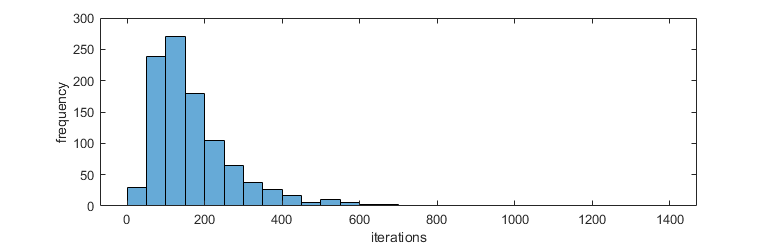
\includegraphics[width=\textwidth]{lab.png}
\end{figure}
\ \\
The bound of $t$ however is not as useful as it should be:
\begin{figure}[H]
	\centering
	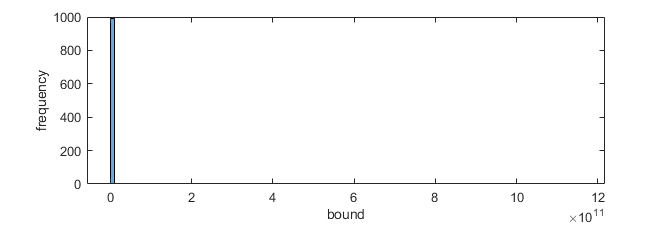
\includegraphics[width=\textwidth]{bound.png}
\end{figure}
\ \\
The average of bounds is $2.0250 \times 10^9$, which is much larger than the actual iterations. This is reasonable, the expected value of bounds is actually calculatable. But I won't do the math here, since the $\text{E}\left(\frac{R^2\mol{\vw^*}^2}{\rho^2}\right)$ is extremly complex and it's not required in this assignment. To calculate this you should at least master the distribution of min value and max value and Chi square distribution. However just give a second thought you can get the idea that why this value tends to be so big, since $\rho$ is a min value, it tend to $0$, and none of $R$ or $\mol{\vw}$ tend to $0$. So I assume that the bound we calculated in problem 1 is merely a math tool to prove the convergence of PLA.
%%%%%%%%%%%%%%%%%%%%%%%%%%%%%%%%%%%%%%%%%%%%%%%%%%%%%%%%%%%%%%%%%%%%%%%%%%%%%%%%%%%%%%%%
\section{3 \wuhao{LED Problem 1.7}}
%%%%%%%%%%%%%%%%%%%%%%%%%%%%%%%%%%%%%%%%%%%%%%%%%%%%%%%%%%%%%%%%%%%%%%%%%%%%%%%%%%%%%%%%
\def\P{\mathbb{P}}
\newcommand{\e}[2]{$#1 \times 10^{#2}$}
\begin{tlist}{4}
	\item[(a)]
	Simply follow $\P=1-\left[1-(1-\mu)^N\right]^{coins}$, we have
	\begin{center}
		\begin{tabular}{|c|c|c|c|}\hline
			\diagbox{$\mu$}{coins} & $1$            & $1000$         & $1000000$ \\\hline
			$0.05$                 & $0.5987$       & $1$            & $1$       \\\hline
			$0.8$                  & \e{1.0240}{-7} & \e{1.0239}{-4} & $0.0973$  \\\hline
		\end{tabular}
	\end{center}
	\item[(b)]
	Since $\P(k)=\left(\begin{array}{c}6\\k\end{array}\right)0.5^6$, the distribution of $v$ should be
	$$
		\begin{array}{c|ccccccc}
			v    & 0      & 1/6    & 1/3    & 1/2    & 2/3    & 5/6    & 1      \\\hline
			P(v) & 0.0156 & 0.0938 & 0.2344 & 0.3125 & 0.2344 & 0.0938 & 0.0156 \\
		\end{array}
	$$
	Denote $w_i = |v_i-\mu_i|$ for $i = 1,2$. the distribution of $w_i$ should be
	$$
		\begin{array}{c|cccc}
			w_i    & 0      & 1/6    & 1/3    & 1/2    \\\hline
			P(w_i) & 0.3125 & 0.4688 & 0.1876 & 0.0312 \\
		\end{array}
	$$
	Then $\P(\max\limits_i w_i>\epsilon)=1-\P(\max\limits_i w_i\leq\epsilon)=1-\P(w_1\leq\epsilon)\P(w_2\leq\epsilon)$. Thus we have
	$$
		\begin{array}{c|cccc}
			\epsilon                      & [0,1/6) & [1/6,1/3) & [1/3,1/2) & [1/2,1) \\\hline
			P(\max\limits_i w_i>\epsilon) & 0.9023  & 0.3896    & 0.0612    & 0       \\
		\end{array}
	$$
	\begin{figure}[H]
		\centering
		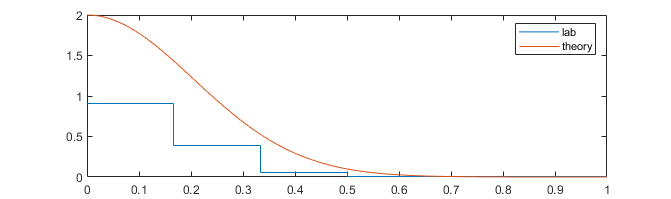
\includegraphics[width=\textwidth]{3.png}
	\end{figure}
\end{tlist}
%%%%%%%%%%%%%%%%%%%%%%%%%%%%%%%%%%%%%%%%%%%%%%%%%%%%%%%%%%%%%%%%%%%%%%%%%%%%%%%%%%%%%%%%
\section{4 \wuhao{LED Problem 1.8}}
%%%%%%%%%%%%%%%%%%%%%%%%%%%%%%%%%%%%%%%%%%%%%%%%%%%%%%%%%%%%%%%%%%%%%%%%%%%%%%%%%%%%%%%%
\def\E{\mathbb{E}}
\begin{tlist}{4}
	\item[(a)]
	Denote the $f(x)$ as the PDF of $t$, we have
	\begin{align*}
		\P\left[t\geq \alpha\right]
		 & =\ \int_\alpha^\infty f(x)dx                        \\
		 & =\ \frac{1}{\alpha}\int_\alpha^\infty \alpha f(x)dx \\
		 & \leq\ \frac{1}{\alpha}\int_\alpha^\infty xf(x)dx    \\
		 & =\ \E(t)/\alpha                                     \\
	\end{align*}
	\item[(b)]
	It's obviously true based on the proof of \textbf{(a)} and $\E\left[(u-\mu)^2\right]=\sigma^2$.
	\item[(c)]
	Based on \textbf{(b)}, and since $u_i$ are iid. we show
	\begin{align*}
		\E\left[(u-\mu)^2\right]
		 & =\ \E\left[\frac{1}{N^2}\left(\sum_{n=1}^N(u_n-\mu)\right)^2\right]                                  \\
		 & =\ \frac{1}{N^2}\E\left[\left(\sum_{n=1}^N(u_n-\mu)^2+\sum_{i\neq j}(u_i-\mu)(u_j-\mu)\right)\right] \\
		 & =\ \frac{1}{N^2}\E\left[\sum_{n=1}^N(u_n-\mu)^2\right]                                               \\
		 & =\ \frac{\sum_{n=1}^N\E(u_n-\mu)^2}{N^2}                                                             \\
		 & =\ \frac{\sigma^2}{N}                                                                                \\
	\end{align*}
	Namely, $\P\left[(u-\mu)^2\geq \alpha\right]\leq\frac{\sigma^2}{N\alpha}$.
\end{tlist}
\end{document}